\chapter{Current APRS Demodulation Approaches}
In the world of APRS there are many solutions that hams use to be able to utilize the network. Some they find and make work, some they purchase to use exclusive for APRS, and some go through the trouble of inventing their own solutions. This chapter explains some of the common systems used on the APRS network, primarily those that can be used for receiving, starting with terminal node controllers and progressing to software based demodulation.

\section{Terminal Node Controllers}
Currently there are many systems that will demodulate these Bell 202 encoded APRS packets. The original hardware used for this communication style was dedicated modems similar to dial-up 56k modems that did the encoding and decoding. These modems were connected directly to the radio and the radio would let the modem know through a signal pin if the radio was receiving what it thought was a data carrying signal. The terminal node controller (TNC), a modem used in AX.25 operation, would let the radio know by signalling the radio to transmit when it had data to send out.

%%%Potentiall needs some editing - TO DO%%%
%As mentioned in the introduction and early in this section, the technologies that are being used for this data transport originated in the late 1980s even though the spec for the protocol itself did not get officially released until 2000. This serves as a reminder that old hardware is commonly used that is not well understood. If a user gets something reasonable working, they will use it without doing a full analysis on edge cases or making simple modification to improve performance.

With a radio and a Terminal Node Controller, amateur packet stations and digipeaters (digital packet repeaters) are possible. Digipeaters are an essential part of the ham packet network, but many users wish to report their GPS position onto the APRS network instead of just relaying traffic for other stations. In order to accomplish this, a GPS receiver is required. Now, stations can take the data from their GPS receiver and put it in the payload of the APRS packet and transmit the GPS reported position onto the network. Within the testing scope of this project there are two TNCs whose decoding results are compared to the software approaches. These two modems are the AEA PK-88 and the Kantronics KAM Plus. However, the PK-88 and the KAM Plus although used very frequently in APRS systems are not fully dedicated hardware for APRS, but instead modems that are being used for ARPS.

\begin{figure}
  \centering
	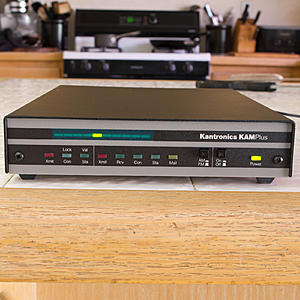
\includegraphics[width=0.75\linewidth]{images/Kantronics-KAM-Plus.jpg} 
	\caption{Image of the Kantronics Kam Plus \cite{KK6RF}}
\end{figure}

\section{Specialized APRS Hardware}
Many people know exactly what they would like to do with APRS and exactly what traffic they want to contribute to the APRS network. This has allowed for companies to start commercially making dedicated APRS hardware, since there is a demand for it. In addition to making this hardware available the produces support the hardware and make pretty user interfaces for the users to be able to program the hardware exactly as they like and without having to invest much time into understanding how different components work together. Some examples of APRS exclusive devices are ArgentData�s OpenTrackers, Byonics� TinyTrack, and Fox Delta�s Fox Track \cite{Miller,Byonics,Foxtrak}. These compact packages along with a radio and a GPS module perform APRS tasks at a satisfactory level for many users.

\begin{figure}
  \centering
	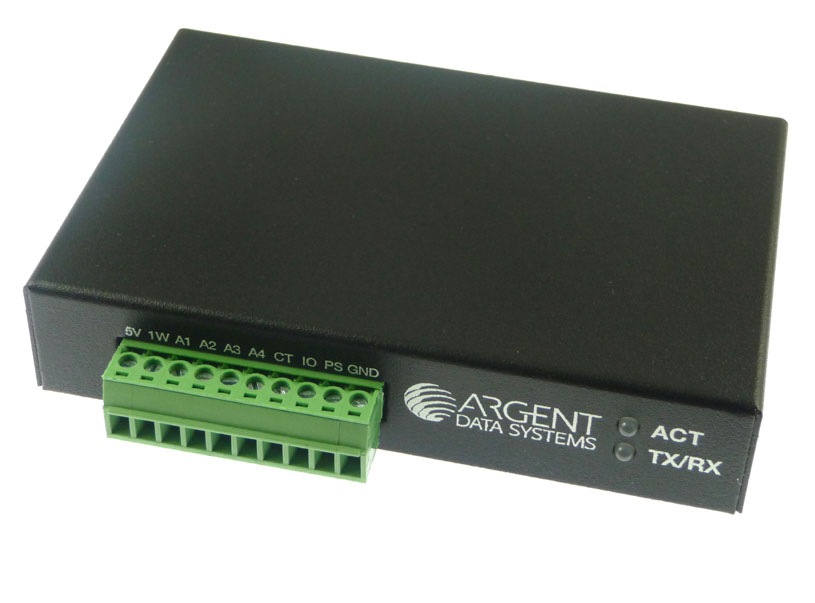
\includegraphics[width=0.75\linewidth]{images/Ot3m-termblk.jpg} 
	\caption{Image of Argent Data's Open Tracker 3. \cite{Data}}
\end{figure}

Since the average user only wants to report positional information, these dedicated devices are simple to setup to do such but also only include a simple feature set. Although these trackers contain some features, since they are basically small embedded systems they do not have all of the features that APRS support. An example is the messaging service. Since these devices don�t have a display or a keypad, there is no way to input or display a message. Certain radio manufacturers have begun to integrating the TNCs into the radios themselves to utilize the radio�s screen. The Kenwood TM-D700 series and Yaesu FTM-350 are examples \cite{Kenwood,Yaesu}.

\begin{figure}
  \centering
	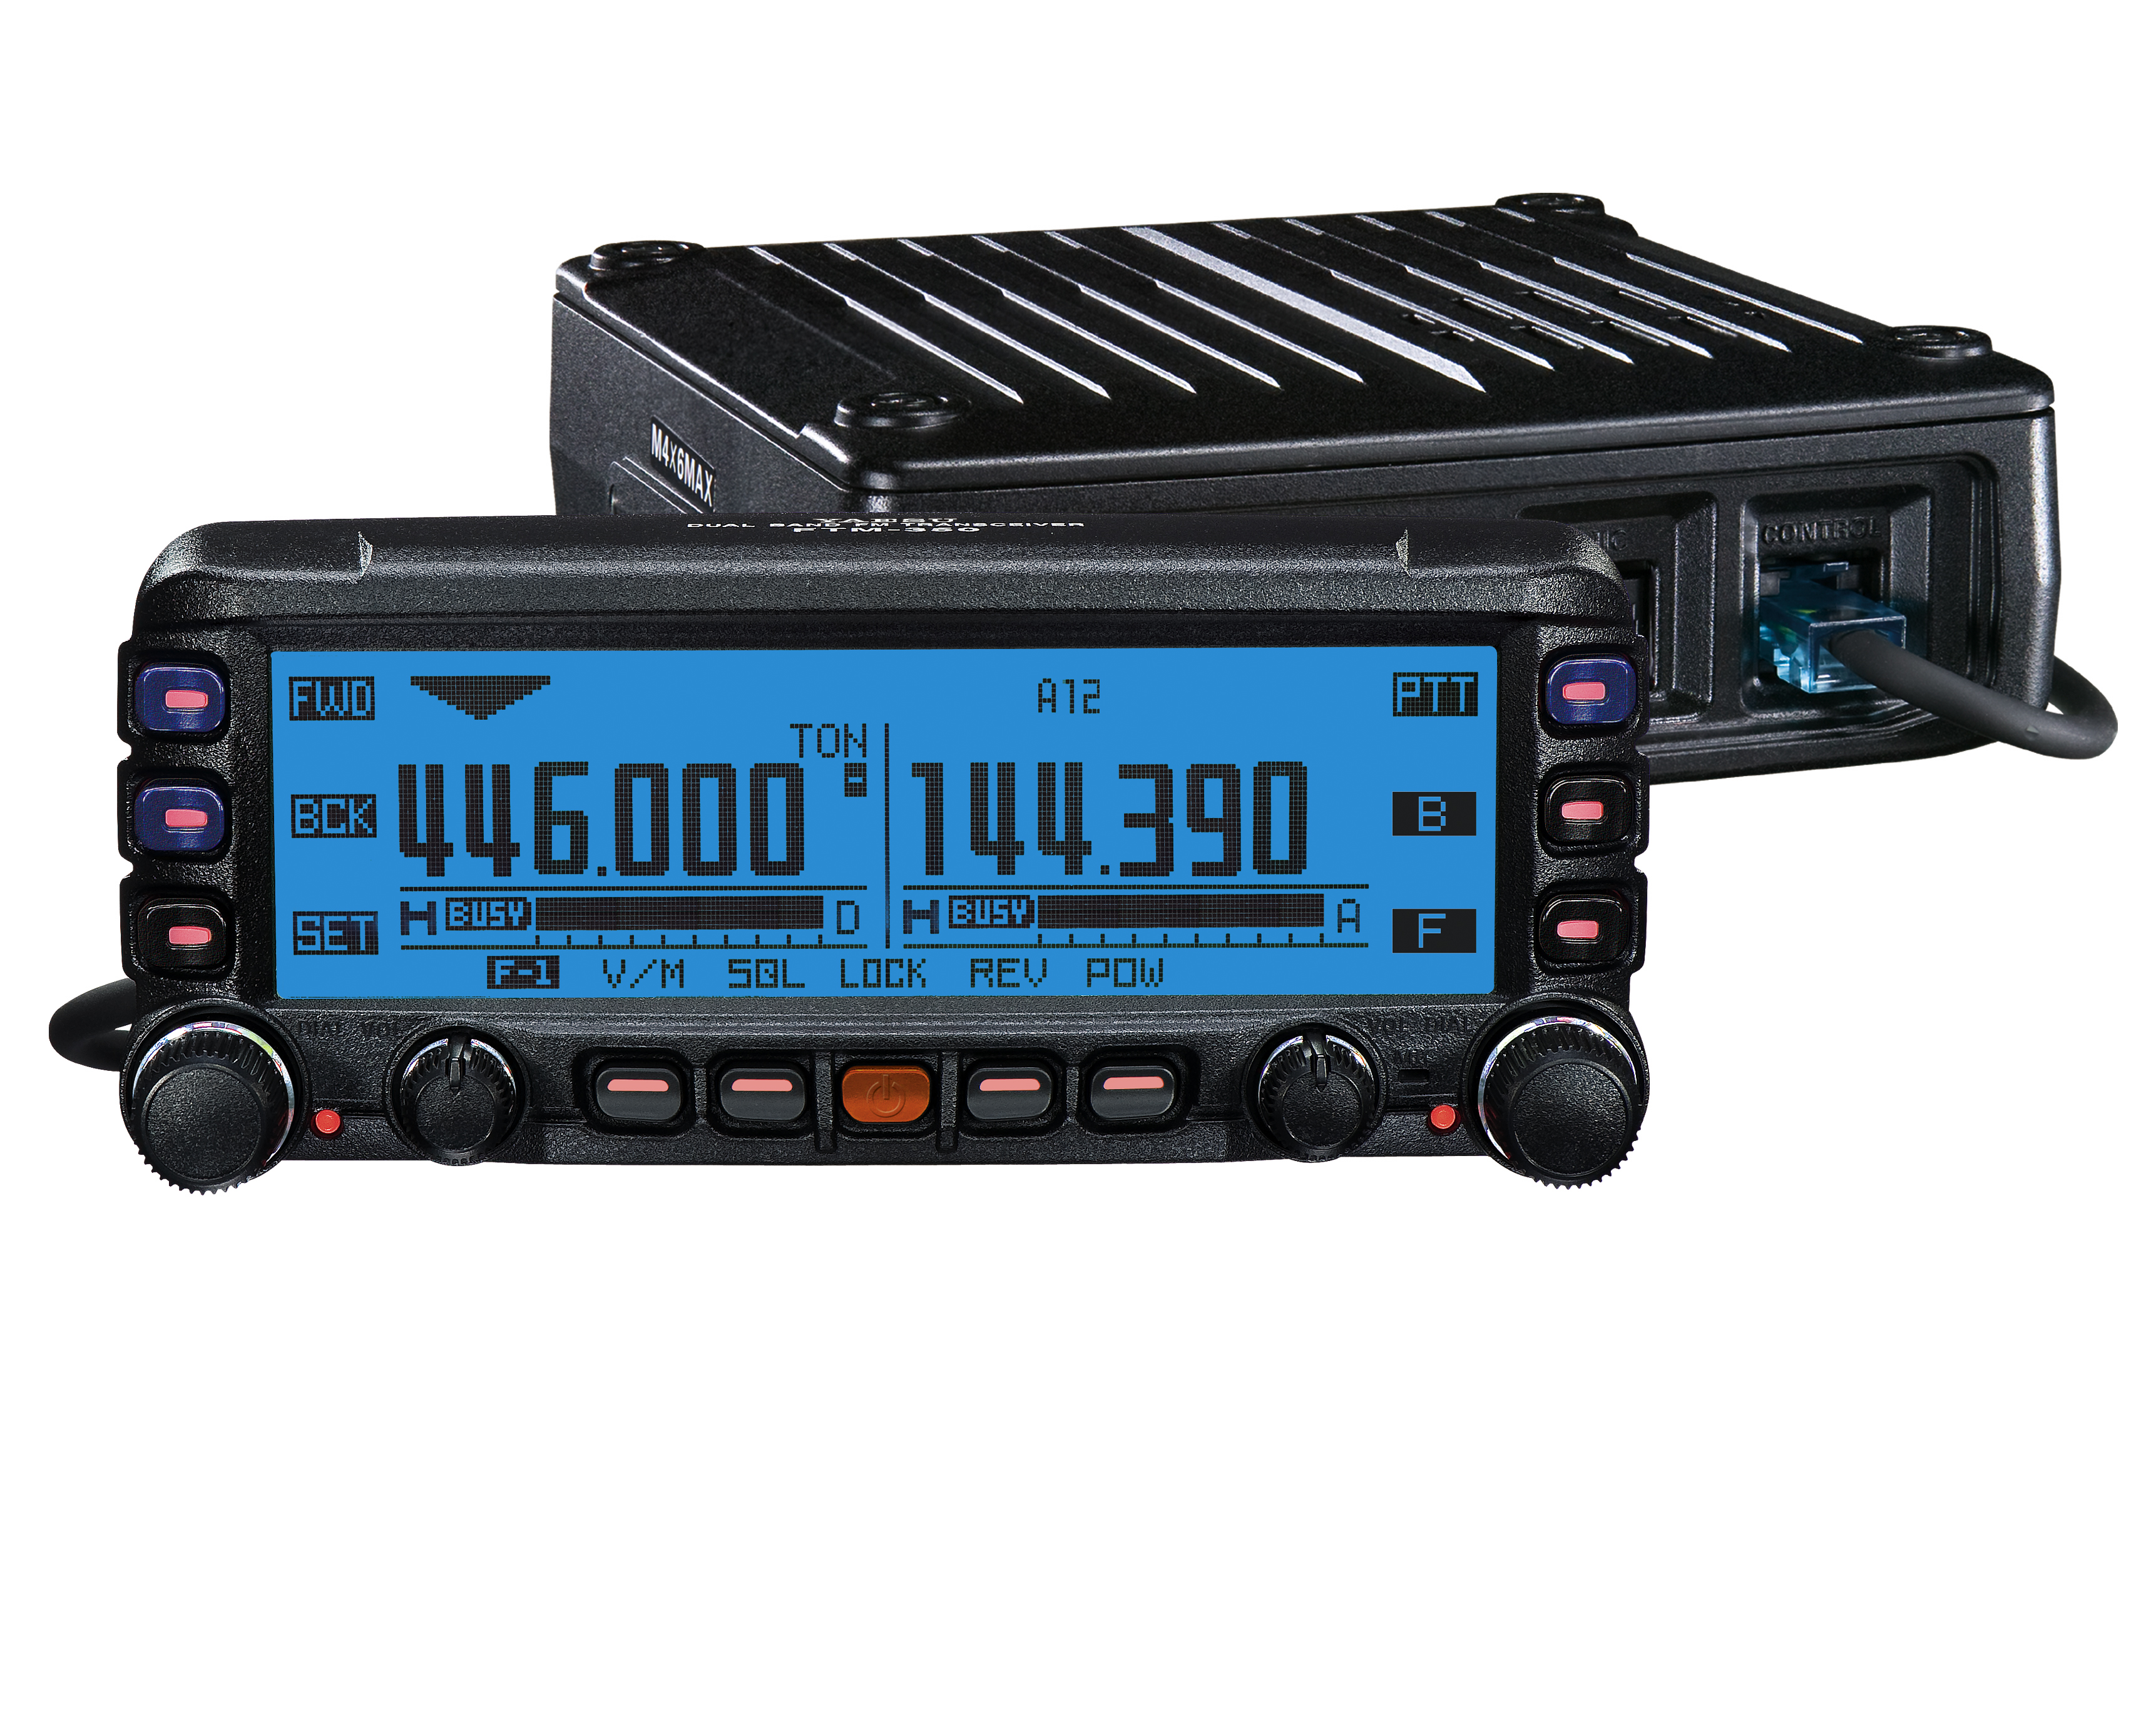
\includegraphics[width=0.75\linewidth]{images/FTM-350US_F.jpg} 
	\caption{Image of the FTM-350 Radio which has APRS integrated. \cite{Yaesua}}
\end{figure}

However, both the options that were presented in this section and the one previous on TNCs require going out and buying special hardware in order to perform APRS whether it be a TNC itself of a OpenTracker. This can be expensive and cost prohibitive for some hams to be able to begin APRS operations.

\section{Software Based Demodulation}
%Copied from old Software Based Demodulation
It can be assumed that before a ham operator becomes interested in the APRS network and sending APRS packets that they will already have a radio. So, if they already have a radio all they have to do is buy a piece of hardware that will do the modulation in order to send a packet. However, hardware costs money and before diving right in it might be nice to get their feet wet first. A good, cheap alternative to dedicated hardware is to use hardware that hams already have. A good choice that will fit the needs is a computer, which most hams probably own at least one of. On this computer amateurs can build or buy a cheap interface to a radio, ~$15 instead of ~$150 for a piece of dedicated hardware, and then use software to do the modulation and demodulation.

This seems to be a route that some are taking and a demodulation scheme that this project explores in detail, but first some more information on current systems that operate in this software realm. Some examples of the software that can be used are George Rossopoylos�s Packet Engine \cite{Rossopoylos} or Thomas Sailer�s Linux Sound Modem \cite{Sailer1997}. On a computer, even ones with minimal resources, there are algorithms that are being used to demodulate the APRS packets. Again, what this project aims to investigate is what improvements can be made to the algorithms and software based demodulation approaches in order to decode these packets in a more robust fashion and to try and get similar performance to TNCs and dedicated hardware. 

Preliminary testing shows that the software still has room for improvement in order to be at least as good as TNCs. As mentioned thus far, software provides a viable low cost alternative to dedicated hardware, but is just that - a cheap solution. It still has some weaknesses that need to be addressed, and refinements to be made to improve demodulation to match performance of hardware. 
%%%MENTION APRS DROID HERE OR IN JAVAAX25 SECTION